\documentclass[twocolumn]{extarticle}
\usepackage{fontspec}   %加這個就可以設定字體
\usepackage{xeCJK}       %讓中英文字體分開設置
\usepackage{indentfirst}
\usepackage{listings}
\usepackage[newfloat]{minted}
\usepackage{float}
\usepackage{graphicx}
\usepackage{caption}
\usepackage{fancyhdr}
\usepackage{hyperref}
\usepackage{amsmath}
\usepackage{multirow}
\usepackage[dvipsnames]{xcolor}
\usepackage{graphicx}
\usepackage{tabularx}
\usepackage{booktabs}
\usepackage{caption}
\usepackage{subcaption}
\usepackage{pifont}
\usepackage{amssymb}
\usepackage{titling}
\usepackage{physics}



\usepackage{pdftexcmds}
\usepackage{catchfile}
\usepackage{ifluatex}
\usepackage{ifplatform}

\usepackage[breakable, listings, skins, minted]{tcolorbox}
\usepackage{etoolbox}
\setminted{fontsize=\footnotesize}
\renewtcblisting{minted}{%
    listing engine=minted,
    minted language=python,
    listing only,
    breakable,
    enhanced,
    minted options = {
        linenos, 
        breaklines=true, 
        breakbefore=., 
        % fontsize=\footnotesize, 
        numbersep=2mm
    },
    overlay={%
        \begin{tcbclipinterior}
            \fill[gray!25] (frame.south west) rectangle ([xshift=4mm]frame.north west);
        \end{tcbclipinterior}
    }   
}

\usepackage[
top=1.5cm,
bottom=0.75cm,
left=1.5cm,
right=1.5cm,
includehead,includefoot,
heightrounded, % to avoid spurious underfull messages
]{geometry} 

\newenvironment{code}{\captionsetup{type=listing}}{}
\SetupFloatingEnvironment{listing}{name=Code}
\usepackage[moderate]{savetrees}


\title{NYCU Introduction to Machine Learning, Homework 2}
\author{110550088 李杰穎}
\date{}


\setCJKmainfont{Noto Serif TC}


\ifwindows
\setmonofont[Mapping=tex-text]{Consolas}
\fi

\XeTeXlinebreaklocale "zh"             %這兩行一定要加,中文才能自動換行
\XeTeXlinebreakskip = 0pt plus 1pt     %這兩行一定要加,中文才能自動換行

\setlength{\parindent}{0em}
\setlength{\parskip}{2em}
\renewcommand{\baselinestretch}{1.25}
\setlength{\droptitle}{-7.5em}   % This is your set screw
\setlength{\columnsep}{2em}
\usepackage{enumitem}

\begin{document}

\maketitle

\section{Part. 1, Coding}
\subsection{Logistic Regression}
\begin{enumerate}
\item Show the hyperparameters (learning rate and iteration) that you used.

\begin{itemize}
	\item Learning rate: $0.01$
	\item Iteration: $1000$
\end{itemize}

Noted that I normalize the training data before training.

\item Show the weights and intercept of your model.

\autoref{fig:wab} shows the weights and intercept of the model.

\item Show the accuracy score of your model on the testing set. The accuracy score should be greater than 0.75.

\autoref{fig:wab} shows the accuracy of the model. The accuracy is $0.7541$, which is greater than $0.75$.

\begin{figure}[H]
\centering
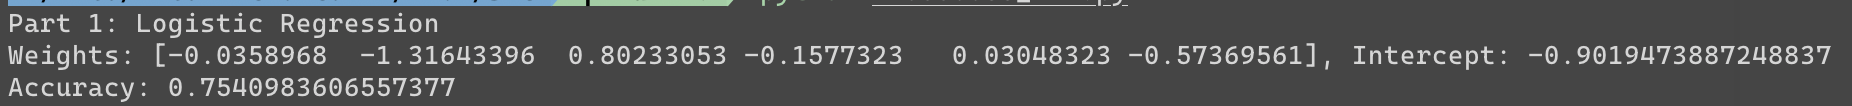
\includegraphics[width=0.95\linewidth]{wab}
\caption{The weights, intercept and accuracy of logistic regression}
\label{fig:wab}
\end{figure}

\end{enumerate}

\subsection{Fisher's Linear Discriminant (FLD)}

\begin{enumerate}
\setcounter{enumi}{3}
\item Show the mean vectors $m_i$ (i=0, 1) of each class of the training set.

\autoref{fig:parafisher} shows the mean vector $m_0$ and $m_1$.

\item Show the within-class scatter matrix $S_W$ of the training set.

\autoref{fig:parafisher} shows the within-class scatter matrix $S_W$ of the training set.

\item Show the between-class scatter matrix $S_B$ of the training set.

\autoref{fig:parafisher} shows the between-class scatter matrix $S_B$ of the training set.

\item Show the Fisher's linear discriminant $w$ of the training set.

\autoref{fig:parafisher} shows the Fisher's linear discriminant $w$.

\item Obtain predictions for the testing set by measuring the distance between the projected value of the testing data and the projected means of the training data for the two classes. Show the accuracy score on the testing set. The accuracy score should be greater than 0.65.

\autoref{fig:parafisher} shows the accuracy on the testing set. The accuracy is $0.657$, which is greater than $0.65$.

\item Plot the projection line (x-axis: age, y-axis: thalach).

\autoref{fig:fisher} shown the projection line.

\begin{figure}[H]
\centering
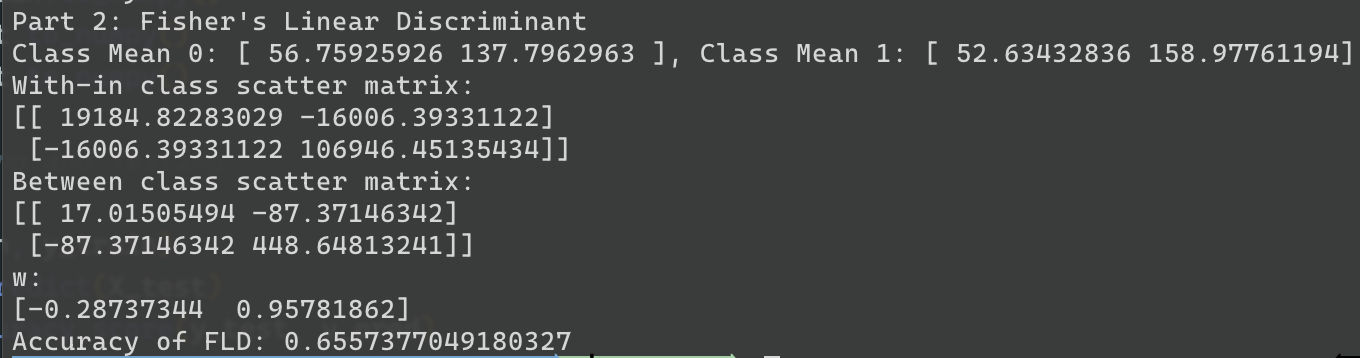
\includegraphics[width=0.95\linewidth]{para_fisher}
\caption{The mean vectors, within-class scatter matrix, between-class scatter matrix, Fisher's linear discriminant and accuracy of FLD method}
\label{fig:parafisher}
\end{figure}


\begin{figure}[H]
\centering
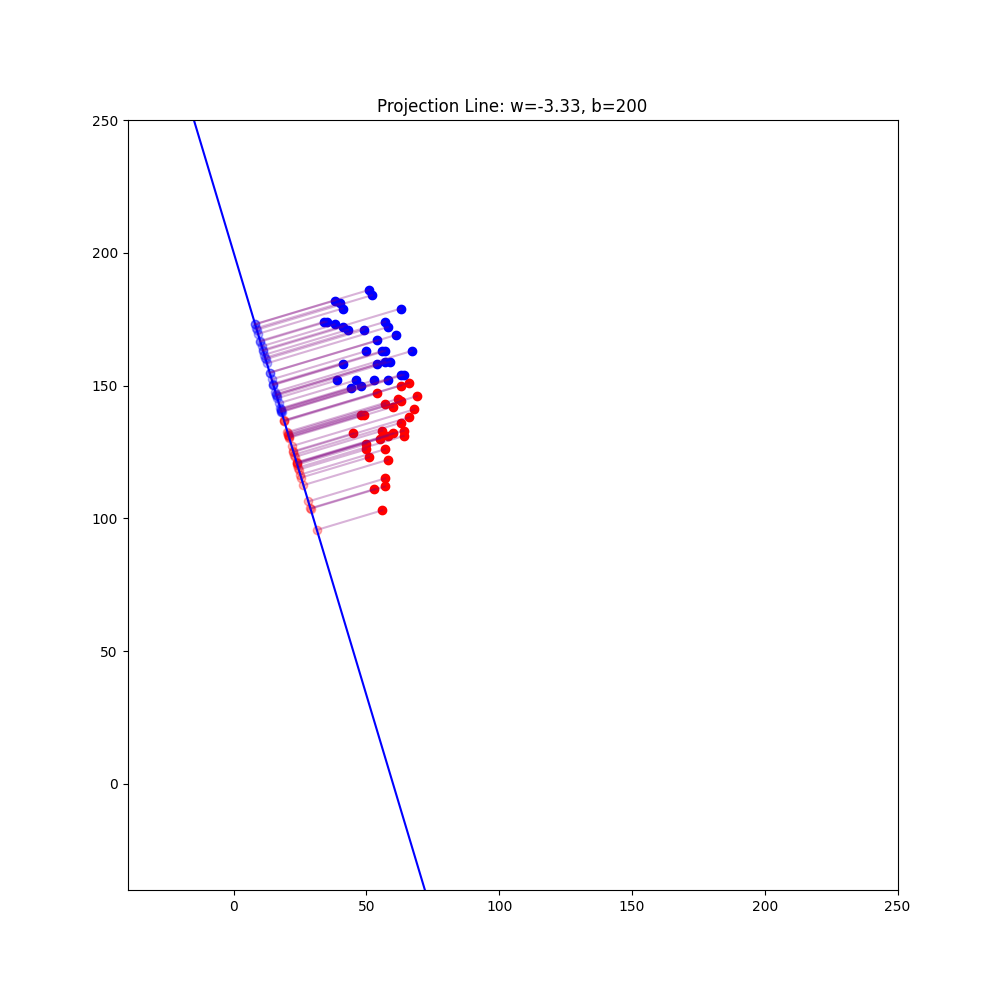
\includegraphics[width=0.95\linewidth]{fisher}
\caption{The projection line given by Fisher's Linear Discriminant. Blue point is positive samples and red is negative samples (x-axis: age, y-axis: thalach)}
\label{fig:fisher}
\end{figure}

\end{enumerate}

\section{Part. 2, Questions}
\begin{enumerate}
\item What's the difference between the sigmoid function and the softmax function? In what scenarios will the two functions be used? Please at least provide one difference for the first question and answer the second question respectively.

First, let's discuss the difference between these two functions from few perspectives:

\begin{itemize}
\item \textbf{Formula}

The sigmoid function is given by $\sigma(x)=\frac{1}{1+e^{-x}}$. In the contrast, the softmax function, for an $n$ dimensional vector $x$, is given by $\text{softmax}(x_i)=\frac{e^{x_i}}{\sum_{j=1}^{n}e^{x_j}}, i=1,2,\dots,n$. Although, the two functions use exponential function, but the mathematical form is quite different.

\item \textbf{Input and output}

The sigmoid function takes any input value $x$ to a value between $0$ and $1$. This function is a non-decreasing and 1-to-1 function, make it useful for model where the output is binary.

And the softmax function converts a vector $x$ to a probability distribution, every value in the converted vector is between 0 and 1, and the sum of all elements is 1.

\end{itemize}

As for the scenarios the two function be used. The sigmoid function is often used in the final layer of a \textbf{binary classification} model to map the single output to probability. For the softmax function, it often used in the final layer of a \textbf{multi-class classification} model to map the output value into a probability for every class.

In summary, the sigmoid function is primarily used for binary classification or scenarios requiring probability estimation for a single event, as for the softmax function, it used in multi-class classification problems where a probabilistic distribution over multiple classes is required.

\item In this homework, we use the cross-entropy function as the loss function for Logistic Regression. Why can't we use Mean Square Error (MSE) instead? Please explain in detail.

First, logistic regression models the probability of a binary outcome. The output of logistic regression, which constraints between 0 and 1, represents the likelihood of a data point belonging to a particular class. However, the MSE loss is designed to measure the average square distance between estimated and actual value, this makes it more suitable for continuous value predictions.

To be more concise, when we apply MSE loss to logistic regression, MSE doesn't reflect the model's performance accurately. The squaring error can lead to small deviation in probabilities are penalized too lightly, and larger deviation too seriously. This make MSE loss often has slower convergence or convergence to local minima when applying to logistic regression.

In the contrast, the cross-entropy function is designed to measure the difference between two probability distributions (e.g. two models whose output is between 0 and 1). Therefore, cross-entropy is a better fit for logistic regression.

Finally, cross-entropy provides a more direct measurement of the model's performance in classification task, compared to MSE. It changes more significantly with small changes in the predicted probabilities, leading to more effective and efficient learning process.



\item In a multi-class classification problem, assume you have already trained a classifier using a logistic regression model, which the outputs are P1, P2, ... Pc, how do you evaluate the overall performance of this classifier with respect to its ability to predict the correct class?

Before answering the three questions below, I assume that P1, P2, ..., Pc are the results after apply softmax function to the original output. This assumption guarantees that the value of $P_{i}$ will between 0 and 1, and $\sum_{i=1}^{c} P_{i} = 1$.

\begin{enumerate}
\item What are the metrics that are commonly used to evaluate the performance of the classifier? Please at least list three of them.

\begin{itemize}
\item Accuracy

This method measure the percentage of correctly predicted instance out of all predictions. It's straightforward but may not be informative in case of class imbalance. We can also calculate the in-class accuracy.

\item Precision, recall and F1-score

Precision is the ratio of correctly predicted observations to the total predicted observations in that class. 

Recall is the ratio of correctly predicted observations to the total true observations in that class.

And F1-score is a metric that combined precision and recall, one model need to achieve high precision and recall at the same time to achieve high F1-score. The formula of F1-score is $2 \times \text{Precision} \times \text{Recall} / (\text{Precision} + \text{Recall})$.


\item Confusion matrix

Confusion matrix is a matrix that provides a detail view for classifier's performance across all the classes, each entry correspond a predicted class and a true class. The number of that entry $C_{ij}$ show that number of samples that being predicted as class $j$ and its true class is class $i$. By observing the confusion matrix, we can know that the model performs worse when classifying which class.

\end{itemize}

\item Based on the previous question, how do you determine the predicted class of each sample?

Predicted class is the corresponding $i$ whose $P_i$ is the highest among all $P$.


\item In a class imbalance dataset (say 90\% of class-1, 9\% of class-2, and 1\% of class-3), is there any problem with using the metrics you mentioned above and how to evaluate the model prediction performance in a fair manner?

For example, for a imbalance dataset, the classifier can always output class-1 to achieve 90\% of accuracy. This make it unfair to evaluate the model by accuracy.

Therefore, we can need to calculate the in-class accuracy or other metrics, and observe the metrics of every class. And for overall model performance, we can use macro-average, micro-average and weighted-average. Marco-average is a straightforward method, it just takes average of the metrics. As for micro-average, it considers the number of samples in every class, i.e. $\text{Precision}_{\text{micro}}=\frac{\sum \text{TP}_i}{\sum (\text{TP}_i+\text{FP}_i)}$, $\text{Recall}_{\text{micro}}=\frac{\sum \text{TP}_i}{\sum (\text{TP}_i+\text{FN}_i)}$. It's easy to check that the total number of false positve sample and the total number of false negative sample is actually the same, they both eqaul to the total number of wrong predictions. Therefore, for micro-average, accuracy, precision, recall and F1-score are all the same. Lastly, for weighted-average, it weights each metrics using the percentages of that class.

By observing different metrics and confusion matrix, we can evaluate the model in a more fair manner.

\end{enumerate}

\item Calculate the results of the partial derivatives for the following equations. (The first one is binary cross-entropy loss, and the second one is mean square error loss followed by a sigmoid function. $\sigma$ is the sigmoid function.)


Before calculating the below results, let's first prove that $\sigma'(x) = \sigma(x) \ (1-\sigma(x))$

\begin{flalign*}
\sigma'(x) &= \dv{\sigma(x)}{x} &&\\
&= \dv{(\frac{1}{1+e^{-x}})}{x} &&\\
&= e^{-x}(1+e^{-x})^{-2} &&\\
&= \frac{e^{-x}}{1+e^{-x}} \ \frac{1}{1+e^{-x}} &&\\
&= (1 - \frac{1}{1+e^{-x}}) \ \frac{1}{1+e^{-x}} &&\\
&= (1-\sigma(x)) \ \sigma(x) &&\\
\end{flalign*}


\begin{enumerate}
\item $\frac{\partial}{\partial x}(-t * \ln (\sigma(x))-(1-t) * \ln (1-\sigma(x)))$

\begin{align*}
&= -t \ \sigma'(x) \ \frac{1}{\sigma(x)} + (1-t) \ \sigma'(x) \ \frac{1}{1-\sigma(x)} \\
&= -t \sigma(x) (1-\sigma(x)) \ \frac{1}{\sigma(x)} + (1-t)  \sigma(x) (1-\sigma(x)) \ \frac{1}{1-\sigma(x)} \\
&= -t (1-\sigma(x)) + (1-t) \sigma(x) \\
&= \sigma(x) - t \\
\end{align*}

\item $\frac{\partial}{\partial x}\left((t-\sigma(x))^2\right)$

\begin{flalign*}
&= -2 \ \sigma'(x) \ (t-\sigma(x)) &&\\
&= -2 \ \sigma(x) (1-\sigma(x))(t-\sigma(x)) &&\\
\end{flalign*}

\end{enumerate}


\end{enumerate}


\end{document}

 